%%%%%%%%%%%%%%%%%%%%%%%%%%%%%%%%%%%%%%%%%%%%%%%%%%%%%%%%%% 
\section{実行実験}\label{chap:experiment}
%%%%%%%%%%%%%%%%%%%%%%%%%%%%%%%%%%%%%%%%%%%%%%%%%%%%%%%%%% 

%%%%%%%%%%%%%%%%%%%%%%%%%%%% 
\begin{table}[t]\footnotesize
  \centering
  \caption{独自に生成した$k$彩色遷移問題のベンチマーク問題}
  \tabcolsep = 1.5mm
  \label{tab:bench_graph}
  \begin{tabular}{lrrr|r}
  グラフ名 & 頂点数 & 辺数 & 彩色数 & 実行可能解の総数 \\ \hline
  1-FullIns\_3 & 30 & 100 & 4 & 50,693,280 \\ 
  le450\_5a & 450 & 5,714 & 5 & 3,840 \\ 
  le450\_5c & 450 & 9,803 & 5 & 120 \\ 
  le450\_5d & 450 & 9,757 & 5 & 960 \\ 
  myciel3 & 11 & 20 & 4 & 12,480 \\ 
  myciel4 & 23 & 71 & 5 & 2,845,658,400 \\ 
  queen5\_5 & 25 & 160 & 5 & 240 \\  
  queen6\_6 & 36 & 290 & 7 & 100,800 \\ 
  queen7\_7 & 49 & 476 & 7 & 20,160 \\
\end{tabular}
\end{table}
%%%%%%%%%%%%%%%%%%%%%%%%%%%% 

%%%%%%%%%%%%%%%%%%%%%%%%%%%% 
\begin{table*}[t]
  \centering
  \scriptsize
  \caption{実験結果: CPU 時間}
  \label{tab:result_time}
  \renewcommand{\arraystretch}{0.6}
  \begin{tabular}{llr|rrrr} \bhline
  問題名 & 到達可能/到達不能 & ステップ長 & \code{changed} & \code{unchanged} & \code{changed_inc} & \code{unchanged_inc} \\ \bhline
  \multicolumn{3}{r|}{} & \multicolumn{2}{c}{基本ソルバー} & \multicolumn{2}{c}{改良ソルバー} \\ \hline
  1-FullIns\_3\_col4\_1 & REACHABLE & 11 & 1.374 & 1.071 & 1.291 & 0.756 \\
  le450\_5a\_col5\_1 & UNREACHABLE & 3,839 & TO & TO & 3.761 & 2.991 \\
  le450\_5a\_col5\_2 & UNREACHABLE & 3,839 & TO & TO & 2.943 & 11.673 \\
  le450\_5a\_col5\_3 & UNREACHABLE & 3,839 & TO & TO & 4.662 & 22.048 \\
  le450\_5a\_col5\_4 & UNREACHABLE & 3,839 & TO & TO & TO & 7.776 \\
  le450\_5a\_col5\_5 & UNREACHABLE & 3,839 & TO & TO & TO & 26.723 \\
  le450\_5a\_col5\_6 & UNREACHABLE & 3,839 & TO & TO & 3.618 & 3.220 \\
  le450\_5a\_col5\_7 & UNREACHABLE & 3,839 & TO & TO & 1318.024 & 8.698 \\
  le450\_5a\_col5\_8 & UNREACHABLE & 3,839 & TO & TO & 3.367 & 18.226 \\
  le450\_5a\_col5\_9 & UNREACHABLE & 3,839 & TO & TO & 2.943 & 2.847 \\ %\hline
  le450\_5a\_col5\_10 & UNREACHABLE & 3,839 & TO & TO & 2.968 & 3.196 \\
  le450\_5c\_col5\_1 & UNREACHABLE & 119 & TO & TO & 2.189 & 2.165 \\
  le450\_5c\_col5\_2 & UNREACHABLE & 119 & TO & TO & 150.018 & 2.148 \\
  le450\_5c\_col5\_3 & UNREACHABLE & 119 & TO & TO & 150.283 & 2.701 \\
  le450\_5c\_col5\_4 & UNREACHABLE & 119 & TO & TO & 152.434 & 2.102 \\
  le450\_5c\_col5\_5 & UNREACHABLE & 119 & TO & TO & 2.209 & 2.114 \\
  le450\_5c\_col5\_6 & UNREACHABLE & 119 & TO & TO & 2.219 & 2.141 \\
  le450\_5c\_col5\_7 & UNREACHABLE & 119 & TO & TO & 151.252 & 2.150 \\
  le450\_5c\_col5\_8 & UNREACHABLE & 119 & TO & TO & 2.878 & 2.176 \\
  le450\_5c\_col5\_9 & UNREACHABLE & 119 & TO & TO & 2.827 & 2.146 \\ %\hline
  le450\_5c\_col5\_10 & UNREACHABLE & 119 & TO & TO & 2.246 & 2.166 \\
  le450\_5d\_col5\_1 & UNREACHABLE & 959 & TO & TO & 2.680 & 5.653 \\
  le450\_5d\_col5\_2 & UNREACHABLE & 959 & TO & TO & 4.097 & 2.621 \\
  le450\_5d\_col5\_3 & UNREACHABLE & 959 & TO & TO & 3.421 & 2.600 \\
  le450\_5d\_col5\_4 & UNREACHABLE & 959 & TO & TO & 155.850 & 6.960 \\
  le450\_5d\_col5\_5 & UNREACHABLE & 959 & TO & TO & 3.294 & 2.618 \\
  le450\_5d\_col5\_6 & UNREACHABLE & 959 & TO & TO & 199.336 & 25.273 \\
  le450\_5d\_col5\_7 & UNREACHABLE & 959 & TO & TO & 3.308 & 12.001 \\
  le450\_5d\_col5\_8 & UNREACHABLE & 959 & TO & TO & 2.695 & 15.224 \\
  le450\_5d\_col5\_9 & UNREACHABLE & 959 & TO & TO & 3.351 & 13.121 \\ %\hline
  le450\_5d\_col5\_10 & UNREACHABLE & 959 & TO & TO & 333.183 & 7.974 \\
  myciel3\_col4\_1 & REACHABLE & 11 & 0.179 & 0.148 & 0.065 & 0.065 \\
  myciel3\_col4\_3 & REACHABLE & 11 & 0.206 & 0.164 & 0.082 & 0.080 \\
  myciel3\_col4\_4 & REACHABLE & 13 & 0.486 & 0.445 & 0.303 & 0.583 \\
  myciel3\_col4\_7 & REACHABLE & 8 & 0.090 & 0.072 & 0.042 & 0.036 \\
  myciel3\_col4\_8 & REACHABLE & 9 & 0.119 & 0.094 & 0.048 & 0.044 \\
  myciel4\_col5\_2 & REACHABLE & 16 & 42.482 & 48.721 & 20.308 & 134.056 \\
  myciel4\_col5\_3 & REACHABLE & 14 & 17.098 & 21.211 & 5.286 & 80.848 \\
  myciel4\_col5\_4 & REACHABLE & 7 & 0.256 & 0.193 & 0.086 & 0.072 \\
  myciel4\_col5\_6 & REACHABLE & 10 & 1.525 & 1.391 & 1.052 & 1.558 \\ %\hline
  myciel4\_col5\_10 & REACHABLE & 17 & 212.682 & 73.646 & 29.999 & 200.068 \\
  queen5\_5\_col5\_1 & UNREACHABLE & 239 & 439.863 & 302.994 & 0.073 & 0.082 \\
  queen5\_5\_col5\_2 & UNREACHABLE & 239 & 437.481 & 301.194 & 0.074 & 0.057 \\
  queen5\_5\_col5\_3 & UNREACHABLE & 239 & 441.161 & 303.136 & 0.073 & 0.589 \\
  queen5\_5\_col5\_4 & UNREACHABLE & 239 & 443.299 & 304.547 & 0.061 & 0.057 \\
  queen5\_5\_col5\_5 & UNREACHABLE & 239 & 441.616 & 302.366 & 0.074 & 0.067 \\
  queen5\_5\_col5\_6 & UNREACHABLE & 239 & 446.811 & 301.201 & 0.061 & 0.149 \\
  queen5\_5\_col5\_7 & UNREACHABLE & 239 & 441.071 & 303.449 & 0.074 & 0.056 \\
  queen5\_5\_col5\_8 & UNREACHABLE & 239 & 442.539 & 303.821 & 0.073 & 0.137 \\
  queen5\_5\_col5\_9 & UNREACHABLE & 239 & 443.353 & 302.952 & 0.074 & 0.066 \\ %\hline
  queen5\_5\_col5\_10 & UNREACHABLE & 239 & 446.027 & 305.350 & 0.073 & 0.058 \\
  queen6\_6\_col7\_1 & UNREACHABLE & 100,799 & TO & TO & 5.375 & 5.488 \\
  queen6\_6\_col7\_2 & UNREACHABLE & 100,799 & TO & TO & 5.337 & 5.292 \\
  queen6\_6\_col7\_3 & UNREACHABLE & 100,799 & TO & TO & 5.345 & 4.390 \\
  queen6\_6\_col7\_4 & UNREACHABLE & 100,799 & TO & TO & 5.714 & 4.358 \\
  queen6\_6\_col7\_5 & UNREACHABLE & 100,799 & TO & TO & 4.274 & 5.178 \\
  queen6\_6\_col7\_6 & UNREACHABLE & 100,799 & TO & TO & 5.403 & 5.129 \\
  queen6\_6\_col7\_7 & UNREACHABLE & 100,799 & TO & TO & 5.219 & 4.418 \\
  queen6\_6\_col7\_8 & UNREACHABLE & 100,799 & TO & TO & 4.300 & 4.389 \\
  queen6\_6\_col7\_9 & UNREACHABLE & 100,799 & TO & TO & 5.365 & 5.407 \\ %\hline
  queen6\_6\_col7\_10 & UNREACHABLE & 100,799 & TO & TO & TO & 4.412 \\
  queen7\_7\_col7\_1 & UNREACHABLE & 20,159 & TO & TO & 2804.714 & 949.947 \\
  queen7\_7\_col7\_2 & UNREACHABLE & 20,159 & TO & TO & 1.342 & 907.100 \\
  queen7\_7\_col7\_3 & UNREACHABLE & 20,159 & TO & TO & 1.586 & 1.499 \\
  queen7\_7\_col7\_4 & UNREACHABLE & 20,159 & TO & TO & TO & 2.768 \\
  queen7\_7\_col7\_5 & UNREACHABLE & 20,159 & TO & TO & 1.622 & 6.052 \\
  queen7\_7\_col7\_6 & UNREACHABLE & 20,159 & TO & TO & 1.803 & 1626.628 \\
  queen7\_7\_col7\_7 & UNREACHABLE & 20,159 & TO & TO & 1.343 & 1.590 \\
  queen7\_7\_col7\_8 & UNREACHABLE & 20,159 & TO & TO & 1.481 & 3.652 \\
  queen7\_7\_col7\_9 & UNREACHABLE & 20,159 & TO & TO & 1224.680 & 3.760 \\ %\hline
  queen7\_7\_col7\_10 & UNREACHABLE & 20,159 & TO & TO & 1.557 & 1.349 \\ \bhline
  \multicolumn{3}{r|}{平均CPU時間} & 223.796 & 151.341 & 101.758 & 59.095 \\ \bhline
  \multicolumn{3}{r|}{解けた問題数} & 21 & 21 & 67 & 71 \\ \bhline
\end{tabular}


\end{table*}
%%%%%%%%%%%%%%%%%%%%%%%%%%%% 

%%%%%%%%%%%%%%%%%%%%%%%%%%%% 
\begin{figure*}[t]
  \centering
  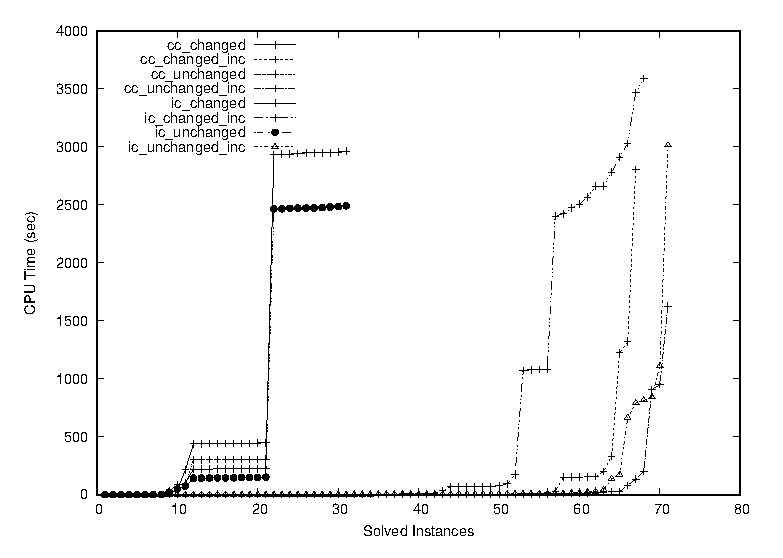
\includegraphics[scale=0.9]{fig/cactus.eps}
  \caption{カクタスプロット}
  \label{fig:cactus}
\end{figure*}
%%%%%%%%%%%%%%%%%%%%%%%%%%%% 

提案した有界組合せ遷移ソルバーの実装方式の性能を評価するために,
$k$彩色遷移問題をベンチマークとして実行実験を行った.
%
ベンチマーク問題には,独自に作成した$k$彩色遷移問題(90問)を使用した.
作成方法は以下の通りである.
\begin{itemize}
\item Graph Coloring and its Generalization~%
  \footnote{\url{https://mat.tepper.cmu.edu/COLOR04/}}
  で公開されているグラフ点彩色問題のインスタンス127個のうち,
  彩色数が判明している44個~\cite{DBLP:journals/constraints/TamuraTKB09}
  をベンチマーク問題の候補とした.
\item 44個のグラフに対して,彩色数での実行可能解の総数を計算できるか調査した.
  総数が得られた9個のグラフを表~\ref{tab:bench_graph}に示す.
\item 総数が得られた9個のグラフについて,
  実行可能解をランダムに2つ選びベンチマーク問題を各10問ずつ作成した(計90問).
\end{itemize}

$k$彩色遷移問題を解く論理プログラムには,
\code{changed}符号化,\code{unchanged}符号化,
\code{changed_inc}符号化,\code{unchanged_inc}符号化
の4つを使用した.
ステップ長の上限値には,解の総数から1ひいた値を使用した
\footnote{ただし,グラフmyciel4から作成した問題については,
{\clingo}が対応している数よりも解の総数が大きかったため,
ステップ長の上限値を$2^{31}-1$とした}.
ASP システムには,{\clingo}のバージョン5.4.0(jumpy)を使用した.
計算環境は Mac OS 3.2GHz 6コア Intel Core i7,64GBメモリである.
1問あたりの制限時間は1時間とした.

表~\ref{tab:result_time}に実験結果を示す.
左から順に問題名,到達可能/到達不能の別,ステップ数,
各符号化の CPU 時間を表している.
解けた問題の数は,
\code{changed}符号化が21問,
\code{unchanged}符号化が21問,
\code{changed_inc}符号化が67問,
\code{unchanged_inc}符号化が71問である.
\code{unchanged_inc}が最も多くの問題を解き,
平均 CPU 時間も最も短い.
%
図~\ref{fig:cactus}にカクタスプロットを示す.
図~\ref{fig:cactus}の縦軸はCPU時間,横軸は解けた問題数を表す.
図より,\code{unchanged_inc}符号化が,他の符号化と比較して,
より多くの問題をより高速に解いていることが確認できる.
以上のことから,インクリメンタルASP解法を用いた有界組合せ遷移ソルバー
の実装方式の有効性が確認できた.
また,\code{changed}符号化と
\code{unchanged}符号化の間に
有意な差が見られた.
これは\code{unchanged}符号化の基礎化後のルール数を
抑えたためと考えられる.

% 本実験により改良ソルバーの手法の有効性が確認できた.
% また,\code{unchanged}符号化の有効性も確認できた.
% これは基礎化によって生成される節数の差によるものと考えられる.
% 基本ソルバーを例とする.
% 2種の符号化において差は遷移制約のみである.
% ステップ長の上限値を$L$,色数を$C$,グラフの頂点数を$V$とすると,
% \code{changed}符号化の遷移制約を基礎化したときの節数が
% $L(2 {}_{C}C_{2} V + 1)$
% であるのに対し,
% \code{unchanged}符号化の同条件の節数は
% $L(CV + 1)$
% である.
% 生成される節数の数が少ない場合,
% 基礎化におけるオーバーヘッドや命題論理として
% 解くときのオーバーヘッドが減少することが考えられる.
% 結果,\code{unchanged}符号化が良い結果を示したと考えられる.

% 本実験で求解できなかった問題に着目すると,
% 1-Fullins\_3, myciel3, myciel4の3個のグラフから生成された
% ベンチマークのみであった.
% これらのグラフは実行可能解の総数が多いという特徴がある.
% これは組合せ遷移問題としての解の探索空間の大きさを意味するため,
% 特に到達可能ではないときの難しさに影響したと考えられる.

%%% Local Variables:
%%% mode: latex
%%% TeX-master: "paper"
%%% End:
